\documentclass[letterpaper, 11pt]{article}

% Standard packages
\usepackage{amsmath, amsthm, latexsym, amssymb, graphicx, color, mathtools, geometry}

% Simplifies margin settings
\usepackage{geometry}
\geometry{margin=1in,headsep=.25in}

% Puts list item indicators in bold; makes flush with previous margin
\renewcommand\labelenumi{\bf\theenumi.}
\renewcommand\labelenumii{\bf\theenumii.}
\setlength\leftmargini{1.4em}
\setlength\leftmarginii{1.4em}

% Flexibility for headers and footers
\usepackage{fancyhdr}
\usepackage{datetime2}


\pagestyle{fancyplain}
\fancyhf{} %clear all header and footer fields
\cfoot{\bf \small Page \thepage}
\headsep 0.2in
\thispagestyle{empty}

\usepackage[pdftex]{hyperref}
\hypersetup{
    unicode=false,          % non-Latin characters in Acrobat's bookmarks
    pdftoolbar=true,        % show Acrobat's toolbar?
    pdfmenubar=true,        % show Acrobat's menu?
    pdffitwindow=true,      % page fit to window when opened
    pdftitle={My title},    % title
    pdfauthor={Author},     % author
    pdfsubject={Subject},   % subject of the document
    pdfnewwindow=true,      % links in new window
    pdfkeywords={keywords}, % list of keywords
    colorlinks=true,        % false: boxed links; true: colored links
    linkcolor=black,        % color of internal links
    citecolor=green,        % color of links to bibliography
    filecolor=magenta,      % color of file links
    urlcolor=blue           % color of external links
}

\renewcommand{\headrulewidth}{0pt}

\parindent 0in
\parskip 12pt

\begin{document}

\title{Homework Template}

\begin{center}
    {
        \large
        \bf
        CS-E4850 Computer Vision\\
        Exercise Round \#2\\
        Submitted by Chen\ Xu, ID 000000\\
        \today
    }
\end{center}

\bigskip

\textbf{Exercise 1. Pinhole camera.}\\

\begin{proof}

    \begin{figure}[!ht]
        \centering
        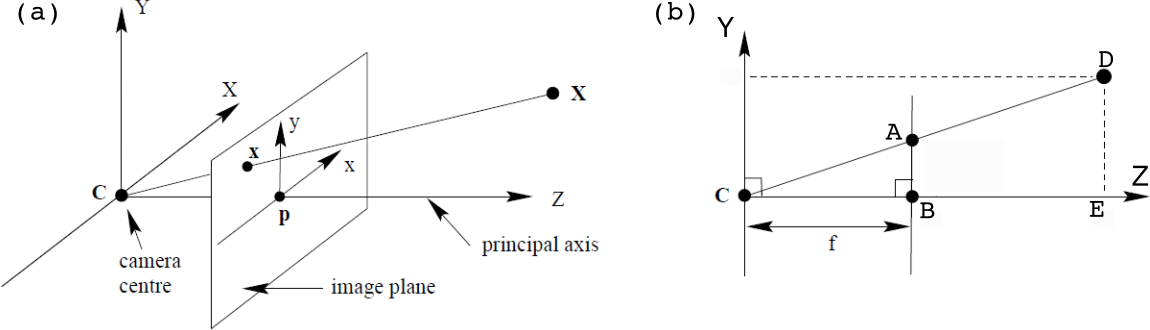
\includegraphics[width=1\textwidth]{pinhole.png}
        \caption{The pinhole model}
        \label{fig:pinhole}
    \end{figure}

    Figure \ref{fig:pinhole}a shows the pinhole model. Figure \ref{fig:pinhole}b shows the projection if one look at the model along the x-axis. Using the rule of similar triangular, one can get:
    \begin{align*}
        \frac{y_p}{y_c}\equiv\frac{|AB|}{|DE|} & = \frac{|CB|}{|CE|}\equiv\frac{f}{z_c} \\
        \therefore y_p                         & = f\frac{y_c}{z_c}
    \end{align*}
    Similarly,
    $$
        x_p = f\frac{x_c}{z_c}
    $$
\end{proof}

\textbf{Exercise 2. Pixel coordinate frame.}\\
\textbf{Solution}\\
a)
$$
    \begin{bmatrix}
        u \\
        v \\
        1
    \end{bmatrix}=
    \begin{bmatrix}
        m_x & 0   & u_0 \\
        0   & m_y & v_0 \\
        0   & 0   & 1
    \end{bmatrix}
    \begin{bmatrix}
        x_p \\
        y_p \\
        1
    \end{bmatrix}$$
b)
$$
    \begin{bmatrix}
        u \\
        v \\
        1
    \end{bmatrix}=
    \begin{bmatrix}
        m_x & - m_x /tan\theta & u_0 \\
        0   & m_y/sin\theta    & v_0 \\
        0   & 0                & 1
    \end{bmatrix}
    \begin{bmatrix}
        x_p \\
        y_p \\
        1
    \end{bmatrix}$$
\textbf{Exercise 3. Intrinsic camera calibration matrix.}\\
$$
    \begin{bmatrix}
        u \\
        v \\
        1
    \end{bmatrix}=
    \begin{bmatrix}
        m_x & 0   & u_0 \\
        0   & m_y & v_0 \\
        0   & 0   & 1
    \end{bmatrix}
    \begin{bmatrix}
        x_p \\
        y_p \\
        1
    \end{bmatrix}
    =
    \begin{bmatrix}
        m_x & 0   & u_0 \\
        0   & m_y & v_0 \\
        0   & 0   & 1
    \end{bmatrix}
    \begin{bmatrix}
        f & 0 & 0 \\
        0 & f & 0 \\
        0 & 0 & 1
    \end{bmatrix}
    \begin{bmatrix}
        x_c \\
        y_c \\
        z_c
    \end{bmatrix}
$$
$$
    \textbf{K}
    =
    \begin{bmatrix}
        m_x & 0   & u_0 \\
        0   & m_y & v_0 \\
        0   & 0   & 1
    \end{bmatrix}
    \begin{bmatrix}
        f & 0 & 0 \\
        0 & f & 0 \\
        0 & 0 & 1
    \end{bmatrix}
    =
    \begin{bmatrix}
        m_x f & 0     & u_0 \\
        0     & m_y f & v_0 \\
        0     & 0     & 1
    \end{bmatrix}
$$

\textbf{Exercise 4. Camera projection matrix.}\\
\begin{align*}
    \textbf{P}_{3 \times 4} & = \textbf{K}\textbf{}{[}\textbf{R}|\textbf{t}\textbf{}{]}=
    \begin{bmatrix}
        m_x f & 0     & u_0 \\
        0     & m_y f & v_0 \\
        0     & 0     & 1
    \end{bmatrix}
    \begin{bmatrix}
        r_{11} & r_{12} & r_{13} & t_1 \\
        r_{21} & r_{22} & r_{23} & t_2 \\
        r_{31} & r_{32} & r_{33} & t_3
    \end{bmatrix}                                                       \\
                            & =
    \begin{bmatrix}
        r_{11} m_x f + u_0 r_{31} & r_{12}m_x f + u_0 r_{32} & r_{13} m_x f + u_0 r_{33} & t_1 m_x f + u_0 t_3 \\
        r_{21} m_y f + v_0 r_{31} & r_{22}m_y f + v_0 r_{32} & r_{23} m_y f + v_0 r_{33} & t_2 m_y f + v_0 t_3 \\
        r_{31}                    & r_{32}                   & r_{33}                    & t_3
    \end{bmatrix}
\end{align*}

\textbf{Exercise 5. Rotation matrix.}\\
a)
\begin{proof}
    \begin{figure}[!ht]
        \centering
        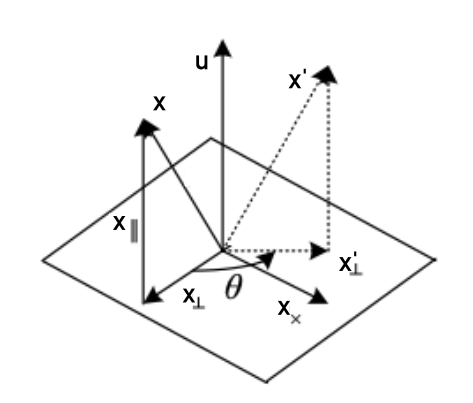
\includegraphics[width=0.6\textwidth]{R2E5.png}
        \caption{Rodrigues Rotation}
        \label{fig:RodriguesRotation}
    \end{figure}
    As it is shown in Figure \ref{fig:RodriguesRotation}, first we project the  vector \textbf{x} onto the axis \textbf{u} to obtain
    \begin{equation}
        \textbf{x}_{\parallel} = \textbf{u}(\textbf{u} \cdot \textbf{x})
    \end{equation}
    which is the component of \textbf{x} that is not affected by the rotation.\\
    Next, we compute the perpendicular residual of \textbf{x} from \textbf{u},
    \begin{equation}
        \textbf{x}_{\perp} = \textbf{x} - \textbf{x}_{\parallel} = \textbf{x} - \textbf{u}(\textbf{u} \cdot \textbf{x})
    \end{equation}
    This vector can rotate around \textbf{u} by $90^{\circ}$ to get
    \begin{equation}
        \textbf{x}_{\times} = \textbf{u} - \textbf{x}_{\perp} = \textbf{u} \times  \textbf{x}
    \end{equation}
    The in-plane component of the rotated vector $\textbf{x}'$ can be calculated as
    \begin{align}
        \textbf{x'}_{\perp} & = cos\theta \textbf{x}_{\perp} + sin\theta \textbf{x}_{\times}\nonumber \\
                            & = cos\theta (\textbf{x} - \textbf{u}(\textbf{u} \cdot \textbf{x})) +
        sin\theta (\textbf{u} \times  \textbf{x})
    \end{align}
    Putting all these terms together, the final rotated vector is
    \begin{align}
        \textbf{R}\textbf{x} & = \textbf{x'} = \textbf{x'}_{\perp} + \textbf{x}_{\parallel} \nonumber \\
                             & = cos\theta (\textbf{x} - \textbf{u}(\textbf{u} \cdot \textbf{x})) +
        sin\theta (\textbf{u} \times  \textbf{x}) +
        \textbf{u}(\textbf{u} \cdot \textbf{x})\nonumber                                              \\
                             & = cos\theta\textbf{x} + sin\theta (\textbf{u} \times  \textbf{x}) +
        (1-cos\theta)(\textbf{u} \cdot \textbf{x})\textbf{u}
    \end{align}
\end{proof}

b)
\textbf{Solution}\\
From a) above
\begin{align*}
    \textbf{R}\textbf{x} & =cos\theta\textbf{x} + sin\theta (\textbf{u} \times  \textbf{x}) +
    (1-cos\theta)(\textbf{u} \cdot \textbf{x})\textbf{u}                                                              \\
                         & = sin\theta \textbf{u} \times  \textbf{x}+cos\theta\textbf{x} +
    (1-cos\theta)(\textbf{u} \cdot \textbf{x})\textbf{u}                                                              \\
                         & = sin\theta \textbf{u} \times  \textbf{x}+ \textbf{x} - \textbf{x} + cos\theta\textbf{x} +
    (1-cos\theta)(\textbf{u} \cdot \textbf{x})\textbf{u}                                                              \\
                         & = sin\theta \textbf{u} \times  \textbf{x}+ \textbf{x} - (1-cos\theta)\textbf{x} +
    (1-cos\theta)(\textbf{u} \cdot \textbf{x})\textbf{u}                                                              \\
                         & = sin\theta \textbf{u} \times  \textbf{x}+ \textbf{x} + (1-cos\theta)(-\textbf{x} +
    (\textbf{u} \cdot \textbf{x})\textbf{u})                                                                          \\
                         & = sin\theta \textbf{u} \times  \textbf{x}+ \textbf{x} + (1-cos\theta)
    \textbf{u} \times (\textbf{u} \times \textbf{x})
\end{align*}
Because $\textbf{u}\times$ can be written as
$$
    \begin{bmatrix}
        0    & -u_3 & u_2  \\
        u_3  & 0    & -u_1 \\
        -u_2 & u_1  & 0
    \end{bmatrix}
$$
The above $\textbf{R}\textbf{x}$ can be written as
\begin{align*}
    \textbf{R}\textbf{x}
     & =
    \textbf{R}
    \begin{bmatrix}
        x_1 \\
        x_2 \\
        x_3
    \end{bmatrix}     \\
     & =
    sin\theta
    \begin{bmatrix}
        0    & -u_3 & u_2  \\
        u_3  & 0    & -u_1 \\
        -u_2 & u_1  & 0
    \end{bmatrix}
    \begin{bmatrix}
        x_1 \\
        x_2 \\
        x_3
    \end{bmatrix}
    +
    \begin{bmatrix} 1 & 0 & 0 \\ 0 & 1 & 0 \\ 0 & 0 & 1 \end{bmatrix}
    \begin{bmatrix}
        x_1 \\
        x_2 \\
        x_3
    \end{bmatrix}     \\
     & + (1-cos\theta)
    \begin{bmatrix}
        0    & -u_3 & u_2  \\
        u_3  & 0    & -u_1 \\
        -u_2 & u_1  & 0
    \end{bmatrix}
    \begin{bmatrix}
        0    & -u_3 & u_2  \\
        u_3  & 0    & -u_1 \\
        -u_2 & u_1  & 0
    \end{bmatrix}
    \begin{bmatrix}
        x_1 \\
        x_2 \\
        x_3
    \end{bmatrix}     \\
     & =
    sin\theta
    \begin{bmatrix}
        0    & -u_3 & u_2  \\
        u_3  & 0    & -u_1 \\
        -u_2 & u_1  & 0
    \end{bmatrix}
    \begin{bmatrix}
        x_1 \\
        x_2 \\
        x_3
    \end{bmatrix}
    +
    \begin{bmatrix} 1 & 0 & 0 \\ 0 & 1 & 0 \\ 0 & 0 & 1 \end{bmatrix}
    \begin{bmatrix}
        x_1 \\
        x_2 \\
        x_3
    \end{bmatrix}     \\
     & + (1-cos\theta)
    \begin{bmatrix}
        u^2_1-1 & u_1 u_2 & u_1 u_3 \\
        u_1 u_2 & u^2_2-1 & u_2 u_3 \\
        u_1 u_3 & u_2 u_3 & u^2_3-1
    \end{bmatrix}
    \begin{bmatrix}
        x_1 \\
        x_2 \\
        x_3
    \end{bmatrix}     \\
     & =
    \begin{bmatrix}
        cos\theta+u^2_1(1-cos\theta)       & u_1 u_2(1-cos\theta)-u_3 sin\theta & u_1 u_3(1-cos\theta)+u_2 sin\theta \\
        u_1 u_2(1-cos\theta)+u_3 sin\theta & cos\theta+u^2_2(1-cos\theta)       & u_2 u_3(1-cos\theta)-u_1 sin\theta \\
        u_1 u_3(1-cos\theta)-u_2 sin\theta & u_2 u_3(1-cos\theta)+u_1 sin\theta & cos\theta+u^2_3(1-cos\theta)
    \end{bmatrix}
    \begin{bmatrix}
        x_1 \\
        x_2 \\
        x_3
    \end{bmatrix}     \\
\end{align*}
Therefore,
$$
    \textbf{R} =
    \begin{bmatrix}
        cos\theta+u^2_1(1-cos\theta)       & u_1 u_2(1-cos\theta)-u_3 sin\theta & u_1 u_3(1-cos\theta)+u_2 sin\theta \\
        u_1 u_2(1-cos\theta)+u_3 sin\theta & cos\theta+u^2_2(1-cos\theta)       & u_2 u_3(1-cos\theta)-u_1 sin\theta \\
        u_1 u_3(1-cos\theta)-u_2 sin\theta & u_2 u_3(1-cos\theta)+u_1 sin\theta & cos\theta+u^2_3(1-cos\theta)
    \end{bmatrix}
$$


%\begin{align*}
%& I'=\frac{n!}{k!(n-k)!}\\
%& \Rightarrow \textbf{l}^\top\textbf{H}^{-1}\textbf{H}\textbf{x}=0\\
%& \Rightarrow \textbf{l}^\top\textbf{H}^{-1}\textbf{x}'=0\\
%& \therefore \textbf{l}'^\top = \textbf{l}^\top\textbf{H}^{-1}\\
%& \Rightarrow \textbf{l}' = (\textbf{l}^\top\textbf{H}^{-1})^\top = \textbf{H}^{-\top}\textbf{l}
%\end{align*}




%Use exponential notation to show that
%\begin{itemize}
%\item $(1+i)^3 = -2-2i$.
%\item $2i(\sqrt{3}+i)(1+i\sqrt{3})=-8$
%\end{itemize}

%\textbf{Solution}\\
%By direct computation we observe that
%\begin{align*}
%(1+i)^3 &= xxx\\
%		&= yyy\\
%        & \vdotswithin{=} \text{ blah, blah, blah}\\
%        &= -2-2i.
%\end{align*}

%Proceeding to the second part, we compute

%etc.

\end{document}
